\Opensolutionfile{ans}[ans/CD3/Muc_7_8]
\section{Mức độ 7,8 điểm}
\setcounter{ex}{0}
\setcounter{dang}{0}
\begin{dang}
	{Định $m$ để GTLN-GTNN của hàm số thỏa mãn điều kiện cho trước}
\end{dang}
\begin{ex}%[2D1K3-2]
	Cho hàm số $y=\dfrac{x+m}{x-1}$ ($m$ là tham số thực) thỏa mãn $\min\limits_{[2;4]} y=3$. Mệnh đề nào dưới đây đúng?
	\choice
	{\True $m>4$}
	{$3<m\leq4$}
	{$m<-1$}
	{$1\leq m<3$}
	\loigiai
	{Ta có $y'=\dfrac{-1-m}{\left(x-1\right)^2}$.\\
	*\textbf{Trường hợp 1:} $-1-m>0 \Leftrightarrow m<-1$ suy ra $y$ đồng biến trên $[2;4]$, suy ra $$\min\limits_{[2;4]} f(x)=f(2)=\dfrac{2+m}{1}=3  \Leftrightarrow m=1 \;\;\text{(loại)}.$$
	*\textbf{Trường hợp 2:} $-1-m<0 \Leftrightarrow m>-1$ suy ra $y$ nghịch biến trên $[2;4]$, suy ra $$\min\limits_{[2;4]} f(x)=f(4)=\dfrac{4+m}{3}=3  \Leftrightarrow m=5 \Rightarrow m > 4.$$
}
\end{ex}
%%==========Câu 2
\begin{ex}%[2D1K3-2]
	Cho hàm số $ y=\dfrac{x+m}{x+1}$ ($m$ là tham số thực) thỏa mãn $\min\limits_{[1;2]} y+\max\limits_{[1;2]} y=\dfrac{16}{3}$. Mệnh đề nào dưới đây đúng?
	\choice
	{\True $m>4$}
	{$2<m\leq 4$}
	{$m\leq 0$}
	{$0<m\leq 2$}
	\loigiai{
	Ta có $y'=\dfrac{1-m}{(x+1)^2}$.\\
*\textbf{Trường hợp 1:} $m<1$ suy ra $y$ đồng biến trên đoạn $[1;2]$, suy ra 
$$\min\limits_{[1;2]} y+\max\limits_{[1;2]} y=\dfrac{16}{3}  \Leftrightarrow y(1)+y(2)=\dfrac{16}{3} \Leftrightarrow \dfrac{m+1}{2}+\dfrac{m+2}{3}=\dfrac{16}{3} \Leftrightarrow m=5 \;\;\text{(loại)}.$$
*\textbf{Trường hợp 2:} $m>1$ suy ra $y$ nghịch biến trên đoạn $[1;2]$, suy ra $$\min\limits_{[1;2]} y+\max\limits_{[1;2]} y=\dfrac{16}{3}  \Leftrightarrow y(2)+y(1)=\dfrac{16}{3} \Leftrightarrow \dfrac{m+2}{2}+\dfrac{m+1}{3}=\dfrac{16}{3} \Leftrightarrow m=5 \;\;\text{(nhận)}.$$
}
\end{ex}
%%==========Câu 3
\begin{ex}%[2D1K3-2]
	Tổng giá trị lớn nhất và giá trị nhỏ nhất của hàm số $y=\dfrac{x+m}{x+1}$ trên đoạn $[1;2]$ bằng 8 ($m$ là tham số thực). Khẳng định nào sau đây là đúng?
	\choice
	{$m>10$}
	{\True $8<m<10$}
	{$0<m<4$}
	{$4<m<8$}
\loigiai
{Ta có: $y'=\dfrac{1-m}{(x+1)^2}$.\\
Nếu $y'<0$ hoặc $y'>0$ nên hàm số đạt giá trị lớn nhất và nhỏ nhất tại $x=1$, $x=2$.\\ 
Theo đề bài ta có: $$\max\limits_{[1;2]} y+\min\limits_{[1;2]} y=8 \Leftrightarrow y(1)+y(2)=8 \Leftrightarrow \dfrac{m+1}{2}+\dfrac{m+2}{3}=8 \Leftrightarrow m=\dfrac{41}{5}\in (8;10).$$
}
\end{ex}
%%==========Câu 4
\begin{ex}%[2D1K3-2]
	Có bao nhiêu giá trị của tham số $m$ để giá trị lớn nhất của hàm số $y=\dfrac{x-m^2-2}{x-m}$ trên đoạn $[0;4]$ bằng $-1$?
	\choice
	{$3$}
	{$2$}
	{\True $1$}
	{$0$}
	\loigiai
	{Tập xác định: $\mathscr{D}=\mathbb{R}\setminus \left\lbrace m\right\rbrace $.\\
	$y'=\dfrac{m^2-m+2}{(x-m)^2}>0,\forall x\neq m$.\\
	Do đó hàm số đồng biến trên mỗi khoảng xác định.\\
	Hàm số đạt giá trị lớn nhất trên đoạn $[0;4]$ bằng $-1$ khi 
	$$\heva{&m < 0\\&f(4) = 1} \Leftrightarrow \heva{&m<0\\&\dfrac{2-m^2}{4-m}=-1} \Leftrightarrow \heva{&m<0\\&m^2+m-6=0} \Leftrightarrow \heva{&m < 0\\&\hoac{&m = 2 \\&m = -3}} \Leftrightarrow m = -3.$$
}
\end{ex}
%%==========Câu 5
\begin{ex}%[2D1K3-2]
	Cho hàm số $y=\dfrac{x+1}{x-m^2}$ ($m$ là tham số thực) thỏa mãn $\min\limits_{[-3;-2]} y=\dfrac{1}{2}$. Mệnh đề nào dưới đây đúng?
	\choice
	{$3<m\leq 4$}
	{\True $-2<m\leq 3$}
	{$m>4$}
	{$m\leq -2$}
	\loigiai{
	Tập xác định: $\mathscr{D}=\mathbb{R}\setminus \left\lbrace m^2\right\rbrace $.\\
	Ta có $y'=\dfrac{-m^2-1}{(x-m)^2}<0,\forall x\in D$ nên hàm số nghịch biến trên từng khoảng xác định.\\
	Do $\min\limits_{[-3;-2]} y=\dfrac{1}{2}=y(-2)=\dfrac{-2+1}{-2-m^2}  \Rightarrow -2-m^2=-2 \Leftrightarrow m=0  \Rightarrow -2<m\leq 3$.
	}
\end{ex}
%%==========Câu 6
\begin{ex}%[2D1K3-2]
	Tìm giá trị dương của tham số $m$ để giá trị nhỏ nhất của hàm số $y=\dfrac{m^2x-1}{x+2}$ trên đoạn $[1;3]$ bằng 1.
	\choice
	{\True $m=\sqrt{2}$}
	{$m=\sqrt{3}$}
	{$m=4$}
	{$m=2$}
	\loigiai{Tập xác định $\mathscr{D}=\mathbb{R}\setminus \left\lbrace -2 \right\rbrace $.\\
	Ta có $y'=\dfrac{2m^2+1}{(x+2)^2}>0, \forall x \neq -2$.\\
Hàm số đồng biến trên đoạn $[1;3]$ nên $\max\limits_{[1;3]} y=y(3) \Leftrightarrow \dfrac{3m^2-1}{5}=1 \Leftrightarrow m=\sqrt{2}$(vì $m>0$).}
\end{ex}
%%==========Câu 7
\begin{ex}%[2D1K3-2]
	Cho hàm số $y=\dfrac{x-m^2}{x+8}$ với $m$ là tham số thực. Giả sử $m_0$ là giá trị dương của tham số $m$ để hàm số có giá trị nhỏ nhất trên đoạn $[0;3]$ bằng $-3$. Giá trị $m_0$ thuộc khoảng nào trong các khoảng dưới đây?
	\choice
	{$(2;5)$}
	{$(1;4)$}
	{$(6;9)$}
	{$(20;25)$}
	\loigiai{
	Tập xác định $D = \mathbb{R} \setminus \{-8\} $.\\
	Ta có $y' = \dfrac{8+m^2}{(x+8)^2} > 0,\forall x \in D$ suy ra hàm số đồng biến trên $[0;3] \Rightarrow \min\limits_{[0;3]} y=y(0)=\dfrac{-m^2}{8}$.\\
	Để $\min\limits_{[0;3]} y=-3 \Leftrightarrow \dfrac{-m^2}{8}=-3 \Leftrightarrow m = \pm 2\sqrt{6} \Rightarrow m_0=2\sqrt{6}\in (2;5)$.
	}
\end{ex}
%%==========Câu 8
\begin{ex}%[2D1K3-2]
	Tìm giá trị của tham số thực $m$ để giá trị nhỏ nhất của hàm số $y=\dfrac{2x+m}{x+1}$ trên đoạn $[0;4]$ bằng $3$.
	\choice
	{$m=3$}
	{$m=1$}
	{\True $m=7$}
	{$m=5$}
	\loigiai
	{Ta có $y'=\dfrac{2-m}{(x+1)^2}$\\
	Nếu $m > 2$ suy ra hàm số nghịch biến trên từng khoảng xác định.\\
	Suy ra $\min\limits_{[0;4]} y=y(4)=\dfrac{m+8}{5} \Rightarrow \dfrac{8+m}{5}=3 \Leftrightarrow m=7$(thỏa mãn).\\
	Nếu $m<2$ suy ra hàm số đồng biến trên từng khoảng xác định.\\
	Suy ra $\min\limits_{[0;4]} y=y(0)=0 \Rightarrow m=3$(loại).\\ Vậy $m=7$.
	}
\end{ex}
%%==========Câu 9
\begin{ex}%[2D1K3-2]
	Tìm các giá trị của tham số $m$ để giá trị nhỏ nhất của hàm số $y=\dfrac{x-m^2+m}{x+1}$ trên đoạn $[0;1]$ bằng $-2$.
	\choice
	{$\hoac{&m=-1\\&m=-2}$}
	{$\hoac{&m=1\\&m=2}$}
	{$\hoac{&m=1\\&m=-2}$}
	{\True $\hoac{&m=-1\\&m=2}$}
	\loigiai{
	Tập xác định $D = \mathbb{R} \setminus \{-1\}$.\\
	Ta có: $y = \dfrac{1 - (-m^2 + m)}{(x + 1)^2} = \dfrac{m^2 - m + 1}{(x + 1)^2} > 0,\forall x \in D \Rightarrow $ hàm số đồng biến trên đoạn $[0; 1]$.\\
	Vậy giá trị nhỏ nhât tại $x=0$ là $y(0)=2 \Leftrightarrow -m^2+m=-2 \Leftrightarrow  \hoac{&m=-1\\&m=2.}$
}
\end{ex}
%%==========Câu 10
\begin{ex}%[2D1K3-2]
	Cho hàm số $y=\dfrac{x+m}{x+1}$ ($m$ là tham số thực) thỏa mãn $\min\limits_{[0;1]} y=3$. Mệnh đề nào dưới đây đúng?
	\choice
	{$1 \leq m<3$}
	{$m>6$}
	{$m<1$}
	{\True $3<m\leq 6$}
	\loigiai
	{Tập xác định $D = \mathbb{R}\setminus \{-1\}$.\\
	Ta có $y'=\dfrac{1-m}{(x+1)^2}$.\\
	*\textbf{Trường hợp 1:} $y'>0 \Leftrightarrow m < 1$ thì $\min\limits_{[0;1]} y=y(0) \Rightarrow m=3$ (loại).\\
	*\textbf{Trường hợp 2:}  $y'<0  \Leftrightarrow m>1$ thì $\min\limits_{[0;1]} y=y(1) \Rightarrow m=5$ (thỏa mãn).
}
\end{ex}
%%==========Câu 11
\begin{ex}%[2D1K3-2]
	Tổng giá trị lớn nhất và giá trị nhỏ nhất của hàm số $y=\dfrac{x+m}{x+1}$ trên $[1;2]$ bằng $8$  ($m$ là tham số thực). Khẳng định nào sau đây đúng?
	\choice 
	{$m>10$}
	{\True $8<m<10$}
	{$0<m<4$}
	{$4<m<8$}
	\loigiai{
	Nếu $m=1$ thì  $y=1$ (không thỏa mãn tổng của giá trị lớn nhất và nhỏ nhất bằng $8$)\\
	Nếu $m\neq 1$ thì hàm số đã cho liên tục trên $[1;2]$  và $y'=\dfrac{1-m}{(x+1)^2}$.\\
	Khi đó đạo hàm của hàm số không đổi dấu trên đoạn $[1;2]$.\\
	Do vậy $\min \limits_{[1;2]}y+\max \limits_{[1;2]}y=y(1)+y(2)=\dfrac{m+1}{2}+\dfrac{m+2}{3}=8\Leftrightarrow m=\dfrac{41}{5}$ .
}
\end{ex}	
\begin{ex}%[2D1K3-2]%Câu 12
	Gọi $A$, $B$ lần lượt là giá trị nhỏ nhất, giá trị lớn nhất của hàm số $y = \dfrac{x + m^2 + m}{x - 1}$ trên đoạn $[2;3]$. Tìm tất cả các giá trị thực của hàm số $m$ để $A + B = \dfrac{13}{2}$.
	\choice
	{\True $m=1;m=-2$}
	{$m=-2$}
	{$m=\pm 2$}
	{$m=-1;m=2$}
	\loigiai{Xét hàm số $y=\dfrac{x+m^2+m}{x-1}$ trên đoạn $[2;3]$.\\
	Ta có $y'=\dfrac{-m^2-m-1}{(x-1)^2}<0, \forall x\in [2;3]$.\\
 	Suy ra $A=f(3)=\dfrac{m^2+m+3}{2}$, $B=f(2)=\dfrac{m^2+m+2}{1}$.\\
 	Khi đó $A + B = \dfrac{13}{2} \Leftrightarrow \dfrac{m^2+m+3}{2}+\dfrac{m^2+m+2}{1}=\dfrac{13}{2} \Leftrightarrow \hoac{&m=2\\&m = -2.}$
}
\end{ex}
%%==========Câu 13
\begin{ex}%[2D1K3-2]
	Cho hàm số $f(x)=\dfrac{x-m^2}{x+8}$ với $m$ là tham số thực. Giả sử $m_0$ là giá trị dương của tham số $m$ để hàm số có giá trị nhỏ nhất trên đoạn $[0;3]$ bằng $-3$. Giá trị $m_0$ thuộc khoảng nào trong các khoảng cho dưới đây?
	\choice
	{$(20;25)$}
	{$(5;6)$}
	{$(6;9)$}
	{\True $(2;5)$}
	\loigiai{
	Xét hàm số $f(x)=\dfrac{x-m^2}{x+8}$ trên đoạn $[0;3]$.\\
	Ta có: $y'=\dfrac{8+m^2}{(x+8)^2}>0, \forall x\in [0;3]$.\\
	Suy ra hàm số $f(x)=\dfrac{x-m^2}{x+8}$ đồng biến trên đoạn $[0;3]$.\\
	Khi đó $\min\limits_{[0;3]} f(x)=f(0)=\dfrac{-m^2}{8}$.\\
	Theo giả thuyết, ta có: $\min\limits_{[0;3]} f(x)=-3 \Leftrightarrow \dfrac{-m^2}{8}=-3 \Leftrightarrow m^2=24 \Rightarrow  \hoac{&m=2\sqrt{6}\\
		&m=-2\sqrt{6} \;\;\text{(loại)}.}$\\
	Vậy $m = 2\sqrt{6} \in (2;5)$.
}
\end{ex}
%%==========Câu 14
\begin{ex}%[2D1K3-2]
	Tìm tất cả các giá trị của tham số $m$ để giá trị nhỏ nhất của hàm số $y=-x^3-3x^2+m$ trên đoạn $[-1;1]$ bằng 0.
	\choice
	{$m=2$}
	{$m=6$}
	{$m=0$}
	{\True $m=4$}
	\loigiai{
	Xét hàm số $y=-x^3-3x^2+m$ trên đoạn $[-1;1]$.\\
	Ta có $y'=-3x^2-6x$.\\
	Khi đó $y'=0 \Leftrightarrow  \hoac{&x=0\in [-1;1]\\&x=-2 \in [-1;1].}$\\
	Mà $\heva{&y'(-1)=m-2\\&y'(0)=m\\&y'(1) = m - 4.}$\\
	Do đó $\min\limits_{[-1;1]} y=-4+m=0 \Leftrightarrow m=4$.\\
	Vậy $m=4$ thỏa yêu cầu bài toán.	
}
\end{ex}
%%==========Câu 15
\begin{ex}%[2D1K3-2]
	Tìm tất cả các giá trị thực của tham số $m$ để hàm số $y=x^3-3x^2+m$ có giá trị nhỏ nhất trên đoạn $[-1;1]$ bằng $\sqrt{2}$.
	\choice
	{$m = \sqrt{2}$}
	{$m = 2 + \sqrt{2}$}
	{\True $m = 4 + \sqrt{2}$}
	{$\hoac{&m = 2 + \sqrt{2}\\&m= 4 + 2\sqrt{2}}$}
	\loigiai{Ta có $y' = 3x^2 - 6x$.\\
	Khi đó $y'=0 \Leftrightarrow  \hoac{&x=0\\&x = 2.}$	\\
	Trên $[-1;1]$ ta có $\heva{&y'(-1)=m-4\\&y'(0)=m&\\&y'(1)=m-2}$ nên $\min\limits_{[-1;1]} f(x)=\sqrt{2} \Leftrightarrow m-4=\sqrt{2} \Leftrightarrow m=4+\sqrt{2}$.
}
\end{ex}
%%==========Câu 16
\begin{ex}%[2D1K3-2]
	Có một giá trị $m_0$ của tham số $m$ để hàm số $y=x^3+\left(m^2+1\right)x+m+1$ đạt giá trị nhỏ nhất bằng 5 trên đoạn $[0;1]$. Mệnh đề nào sau đây là đúng?
	\choice
	{\True $2018m_0-m^2_0 \geq 0$}
	{$2m_0-1<0$}
	{$6m_0-m^2_0<0$}
	{$2m_0+1<0$}
	\loigiai{
	Đặt $f(x)=x^3+(m^2+1)x+m+1$.\\
	Ta có: $y'=3x^2+m^2+1>0, \forall x \in \mathbb{R} \Rightarrow $ hàm số đồng biến trên $[0;1]$.\\
	Vì thế $\min\limits_{[0;1]} f(x)=f(0)=m+1$.\\
	Theo bài ta có: $m+1=5 \Rightarrow m=4$.\\
	Vậy nên $m_0=4$ và mệnh đề đúng là $2018m_0-m^2_0\leq 0$.
}
\end{ex}
%%==========Câu 17
\begin{ex}%[2D1K3-2]
	Nếu hàm số $y=x+m+\sqrt{1-x^2}$ có giá trị lớn nhất bằng $2\sqrt{2}$ thì giá trị của $m$ là
	\choice
	{$\dfrac{\sqrt{2}}{2}$}
	{$-\sqrt{2}$}
	{\True $\sqrt{2}$}
	{$-\dfrac{\sqrt{2}}{2}$}
	\loigiai{
	Xét hàm số $y=x+m+\sqrt{1-x^2}$ xác định trên $[-1;1]$.\\
	Ta có: $y'=1-\dfrac{x}{\sqrt{1-x^2}}$.\\
	Khi đó
	$y'=0 \Leftrightarrow  \heva{&\sqrt{1-x^2}=x\\&1-x^2>0} \Leftrightarrow \hoac{&\heva{&1>x\geq 0\\&1-x^2=x}\\&\heva{&1>x \leq 0\\&2x^2=1}} \Leftrightarrow
	\heva{&1>x \geq 0\\&\hoac{&x = \dfrac{1}{\sqrt{2}}\\&x = -\dfrac{1}{\sqrt{2}}}}
 	\Leftrightarrow x=\dfrac{1}{\sqrt{2}}$.	\\
	Ta có $y(-1)=-1+m$, $y(1)=1+m$, $y\left(\dfrac{1}{\sqrt{2}}\right)=\sqrt{2+m}$.\\
	Do hàm số $y$ liên tục trên $[-1;1]$ nên $\max\limits_{[-1;1]} y=m+\sqrt{2}$.\\
	Theo đề bài thì $\max\limits_{[-1;1]} y=2\sqrt{2} \Rightarrow m+\sqrt{2}=2\sqrt{2} \Leftrightarrow m=\sqrt{2}$.
}
\end{ex}
%%==========Câu 18
\begin{ex}%[2D1K3-2]
	Cho hàm số $y=2x^3-3x^2-m$. Trên $\left[-1;1\right]$ hàm số có giá trị nhỏ nhất là $-1$. Tính $m$.
	\choice
	{$m=-6$}
	{$m=-3$}
	{\True $m=-4$}
	{$m=-5$}
	\loigiai{
	Ta có $y'=6x^2-6x$.\\
	Khi đó $y'=0 \Leftrightarrow 6x^2-6x=0 \Leftrightarrow \hoac{&x=0\in [-1;1]\\&x=1 \in [-1;1]}$.\\
	Khi đó $y(-1)=-5-m$. $y(0)=-m$; $y(1)=-1-m \Rightarrow \min\limits_{[-1;1]} y=-5-m$.\\
	Theo đề bài ta có $-5-m=-1 \Leftrightarrow m=-4$.
}
\end{ex}
%%==========Câu 19
\begin{ex}%[2D1K3-2]
	Biết $S$ là tập giá trị của $m$ để tổng giá trị lớn nhất và giá trị nhỏ nhất của hàm số $y=x^4-m^2x^3-2x^2-m$ trên đoạn $[0;1]$ bằng $-16$. Tính tích các phần tử của $S$.
	\choice
	{$2$}
	{$-2$}
	{\True $-15$}
	{$-17$}
	\loigiai{
	Tập xác định $\mathscr{D}=\mathbb{R}$.\\
	Ta có: $y'=4x^3-3m^2x^2-4x$.\\
	Khi đó $y'=0 \Leftrightarrow 4x^3-3m^2x^2-4x=0 \Leftrightarrow \hoac{&x=0\\&4x^2-3m^2x-4=0} \Leftrightarrow \hoac{&x=0\\&x=\dfrac{3m^2+\sqrt{9m^4+64}}{8}>1\\&x=\dfrac{3m^2-\sqrt{9m^4-64}}{8}<0.}$\\
	Nên hàm số đơn điệu trên $(0;1)$.\\
	Tổng giá trị lớn nhất và giá trị nhỏ nhất của hàm số trên đoạn $[0;1]$ bằng $-16$ nên $$y(0)+y(1)=-16 \Leftrightarrow -m+(-m^2-m-1)=-16 \Leftrightarrow -m^2-2m+15=0.$$
	Vậy $m_1 \cdot m_2=-15$.
}
\end{ex}
%%==========Câu 20
\begin{ex}%[2D1K3-2]
	Tìm tất cả giá trị thực của tham số $m$ để hàm số $y=\dfrac{x^2+mx+1}{x+m}$ liên tục và đạt giá trị nhỏ nhất trên đoạn $[0;2]$ tại một điểm $x_0\in (0;2)$.
	\choice
	{\True $0<m<1$}
	{$m>1$}
	{$m>2$}
	{$-1<m<1$}
	\loigiai{
	Tập xác định: $\mathscr{D}=\mathbb{R}\setminus \{-m\}$.\\
	 Hàm số liên tục trên $[0;2]$ nên $\hoac{&-m<0\\&-m>2} \Leftrightarrow \hoac{&m > 0\\&m < -2.}$\\
	Ta có: $y' = \dfrac{x^2+2mx+m^2-1}{(x+m)^2} = \dfrac{(x+m)^2-1}{(x+m)^2}$.\\
	Khi đó $y' = 0 \Leftrightarrow \hoac{&x_1=-m-1\\&x_2=-m+1.}$\\
	Ta có bảng biến thiên
	\begin{center}
	\begin{tikzpicture}
	\foreach \x/\texn in {0/$x$,
	2/$-\infty$,4/$x_1$,7/$-m$,9/$0$,10/$x_2$,11/$2$,12/$+\infty$} \path
	(\x,3.5)node{\texn};
	\foreach \x/\texn in
	{0/$f’(x)$,3/$-$,4/$0$,5/$+$,6/ ,8/$-$,10/$0$,12/$+$} \path
	(\x,2.5)node{\texn};
	\foreach \x/\y/\texn in {0/1/$f(x)$,
	2/.5/$-\infty$,4/1.5/CĐ,6/0.5/$-\infty$,8/1.5/$+\infty$,10/0.5/CT,12/1.5/$+\infty$}
	\path (\x,\y) node(\x){\texn};
	\draw[-stealth] (2)--(4);
	\draw[-stealth](4)--(6);
	\draw[-stealth](8)--(10);
	\draw[-stealth](10)--(12);
	\draw (7,3)--(7,0);
	\draw (7.1,3)--(7.1,0);
	\draw[dashed] (9,3)--(9,0);
	\draw[dashed] (11,3)--(11,0);
	\draw
	(-.5,3)--(12.5,3) (1,4)--(1,0)
	(-.5,2)--(12.5,2)
	(-.5,4) rectangle (12.5,0)
	;
	\end{tikzpicture}
	\end{center}
	Hàm số đạt giá trị nhỏ nhất tại $x_0 \in (0;2)$ nên $0<-m+1<2 \Leftrightarrow -1<m<1$.\\
	So với điều kiện hàm số liên tục trên đoạn $[0;2]$.\\
	Vậy ta có $0<m<1$.
}
\end{ex}
%%%%-Câu 21
\begin{ex}%[2D1K3-2]
	Cho hàm số $y=\dfrac{1-m\sin x}{\cos x +2}$. Có bao nhiêu giá trị nguyên của tham số $m$ thuộc đoạn  $[0;10]$ để giá trị nhỏ nhất của hàm số nhỏ hơn $-2$?
	\choice 
	{$1$}
	{$9$}
	{$3$}
	{\True $6$}
	\loigiai{
	Tập xác định: $\mathscr{D}=\mathbb{R}$.\\
	Ta có $y=\dfrac{1-m\sin x}{\cos x+2}\Leftrightarrow y\cos x+m\sin x=1-2y$.\\
	Phương trình có nghiệm khi và chỉ khi $y^2+m^2\geq 1-4y+4y^2\Leftrightarrow 3y^2-4y+1-m^2\leq 0\Leftrightarrow \dfrac{2-\sqrt{1+3m^2}}{3}\leq y\leq \dfrac{2+\sqrt{1+3m^2}}{3}$.\\ 
	Theo đề bài, ta có $\heva{&\min \limits_{x\in \mathbb{R}}y=\dfrac{2-\sqrt{1+3m^2}}{3}<-2\\&m\in [0;10]\\&m\in \mathbb{Z}}\Leftrightarrow \heva{&\sqrt{1+3m^2}>8\\&m\in [0;10]\\&m\in \mathbb{Z}}\Leftrightarrow \heva{&3m^2>63\\&m\in [0;10]\\&m\in \mathbb{Z}}\Leftrightarrow \heva{&m^2>21\\&m\in [0;10]\\&m\in \mathbb{Z}}\Leftrightarrow m\in \{5;6;7;8;9;10\}$.\\
	Vậy có $6$  giá trị nguyên của tham số $m$ thỏa yêu cầu bài toán.
}
\end{ex}
%%%%-Câu 22
\begin{ex}%[2D1K3-2]
	Cho hàm số $y=ax^3+cx+d$, $a\neq 0$ có $\min \limits_{x\in (-\infty;0)} f(x)=f(-2)$. Giá trị lớn nhất của hàm số $y=f(x)$ trên đoạn $[1;3]$ bằng
	\choice 
	{$d-11a$}
	{\True $d-16a$}
	{$d+2a$}
	{$d+8a$}
	\loigiai{
	Vì $y=ax^3+cx+d$ là hàm số bậc ba và có $\min \limits_{x\in (-\infty;0)} f(x)=f(-2)$ nên $a<0$  và $y'=0$  có hai nghiệm phân biệt.\\
	Ta có $y'=3ax^2+c$ có hai nghiệm phân biệt $\Leftrightarrow ac<0$.\\
	Vậy với $a<0$, $c>0$  thì $y'=0$  có hai nghiệm đối nhau $x=\pm \sqrt{-\dfrac{c}{3a}}$.\\ 
	Từ đó suy ra   $\min \limits_{x\in (-\infty;0)} f(x)=f\left(-\sqrt{-\dfrac{c}{3a}}\right)\Leftrightarrow -\sqrt{-\dfrac{c}{3a}}=-2\Leftrightarrow \sqrt{-\dfrac{c}{3a}}=2\Leftrightarrow c=-12a$.\\
	Ta có bảng biến thiên
	\begin{center}
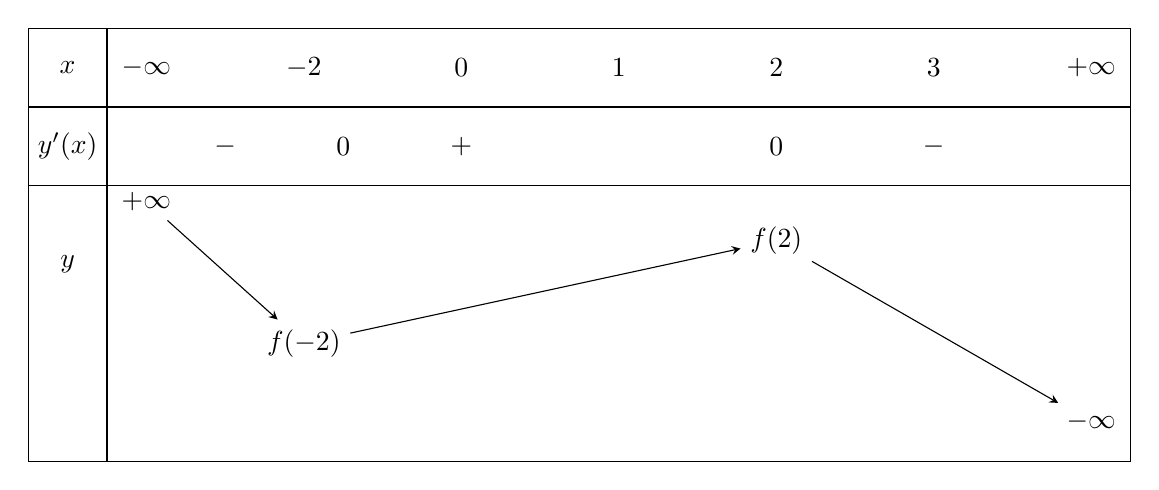
\begin{tikzpicture}
	\foreach \x/\texn in {-4/x,
		-3/-\infty,-1/-2,1/0, 3/1, 5/2, 7/3,9/+\infty} \path
	(\x,3.5)node{$\texn$};
	\foreach \x/\texn in
	{-4/y'(x),-2/-,-0.5/0,1/+,5/0,7/-} \path
	(\x,2.5)node{$\texn$};
	\foreach \x/\y/\texn in {-4/1/y,
		-3/1.8/+\infty,-1/0/f(-2),5/1.3/f(2),9/-1/-\infty}
	\path (\x,\y) node(\x){$\texn$};
	\draw[-stealth] (-3)--(-1);
	\draw[-stealth](-1)--(5);
	\draw[-stealth] (5)--(9);
	\draw
	(-4.5,4)--(9.5,4) (-3.5,4)--(-3.5,-1.5)
	(-4.5,3)--(9.5,3) (-4.5,2)--(9.5,2)
	(-4.5,4) rectangle (9.5,-1.5);
\end{tikzpicture}
\end{center}
	Ta suy ra $\max \limits_{x\in [1;3]} f(x)=f(2)=8a+2c+d=-16a+d$.
}
\end{ex}
%%%%-Câu 23
\begin{ex}%[2D1K3-2]
	Tìm tất cả các giá trị của tham số 	$m$ để hàm số $y=\dfrac{x+m}{x^2+x+1}$ có giá trị lớn nhất trên $\mathbb{R}$  nhỏ hơn hoặc bằng $1$.
	\choice
	{$m\leq 1$}
	{$m\geq 1$}
	{$m\geq -1$}
	{$m\leq -1$}
	\loigiai{
	Tập xác định $\mathscr{D}=\mathbb{R}$.\\
 $\lim\limits_{x\to \infty}y=0$.\\
$y'=\dfrac{-x^2-2mx+1-m}{\left(x^2+x+1\right)^2}$.\\
 $y'=0\Leftrightarrow -x^2-2mx+1-m=0$\\
 Có $\Delta ' =m^2-m+1>0$, $\forall m\in \mathbb{R}$ nên $(*)$ có $2$ nghiệm phân biệt $x_1<x_2$, $\forall m\in \mathbb{R}$.\\
 Bảng biên thiên
 \begin{center}
 	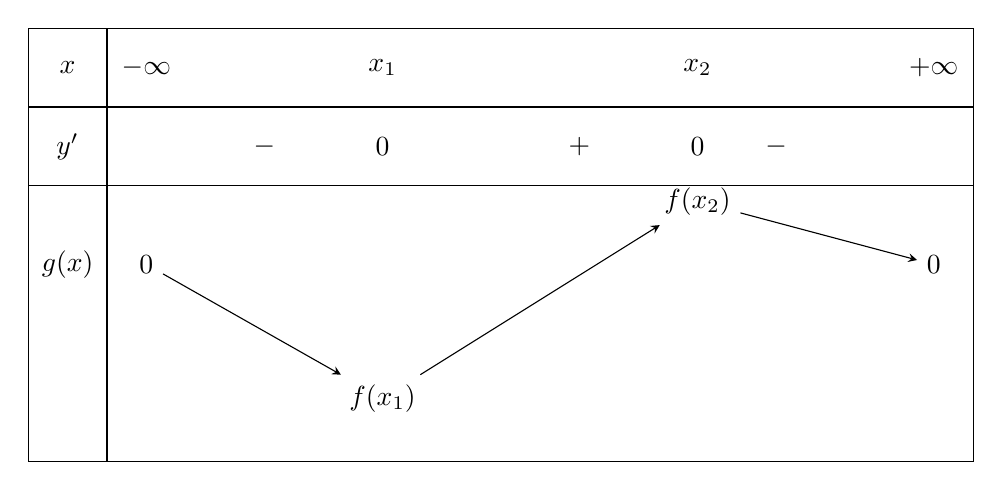
\begin{tikzpicture}
 		\foreach \x/\texn in {-4/x,
 			-3/-\infty,0/x_1,4/x_2, 7/+\infty} \path
 		(\x,3.5)node{$\texn$};
 		\foreach \x/\texn in
 		{-4/y',-1.5/-,0/0,2.5/+,4/0,5/-} \path
 		(\x,2.5)node{$\texn$};
 		\foreach \x/\y/\texn in {-4/1/g(x),
 			-3/1/0,0/-0.7/f(x_1),4/1.8/f(x_2),7/1/0}
 		\path (\x,\y) node(\x){$\texn$};
 		\draw[-stealth] (-3)--(0);
 		\draw[-stealth](0)--(4);
 		\draw[-stealth] (4)--(7);
 		\draw
 		(-4.5,4)--(7.5,4) (-3.5,4)--(-3.5,-1.5)
 		(-4.5,3)--(7.5,3) (-4.5,2)--(7.5,2)
 		(-4.5,4) rectangle (7.5,-1.5);
 	\end{tikzpicture}
 \end{center}
Vậy hàm số đạt giá trị lớn nhất là $f\left(x_2\right)=\dfrac{1}{2x_2+1}$ với $x_2=-m+\sqrt{m^2-m+1}$.\\
 Theo yêu cầu bài toán $\dfrac{1}{-2m+2\sqrt{m^2-m+1}+1}\leq 1\Leftrightarrow 1-2m++2\sqrt{m^2-m+1}\geq 1$ (vì $f\left(x_2\right)>0\Rightarrow 2x_2+1>0$) $\Leftrightarrow \sqrt{m^2-m+1}\geq m\Leftrightarrow \hoac{&m<0\\&\heva{&m\geq 0\\&m^2-m+1\geq m^2}}\Leftrightarrow m\leq 1$.}
\end{ex}
%%%%-Câu 24
\begin{ex}%[2D1K3-2]
	Giá trị lớn nhất của hàm số $y=\dfrac{x^3+x^2-m}{x+1}$  trên $[0;2]$  bằng $5$. Tham số $m$ nhận giá trị là
	\choice 
	{$-5$}
	{$1$}
	{\True $-3$}
	{$-8$}
	\loigiai{
				Tập xác định của hàm số $\mathscr{D}=\mathbb{R}\setminus \{1\}\Rightarrow [0;2]\subset \mathscr{D}$.\\
			Ta có $y=\dfrac{x^3+x^2-m}{x+1}\Rightarrow y'=\dfrac{2x^3+4x^2+2x+m}{\left(x+1\right)^2}$.\\
			$y'=0\Leftrightarrow 2x^3+4x^2+2x+m=0\Leftrightarrow -\left(2x^2+4x^2+2x\right)=m \, (1)$.\\
			Ta có $y(0)=m$, $y(2)=4-\dfrac{m}{3}$.\\ 
			Đặt $g(x)=-\left(2x^3+4x^2+2x\right)\Rightarrow g'(x)=-\left(6x^2+8x+2\right)=0\Leftrightarrow\hoac{&x=-1\\&x=-\dfrac{1}{3}.}$ .
			Trên $[0;2]$  ta có bảng biến thiên
			\begin{center}
				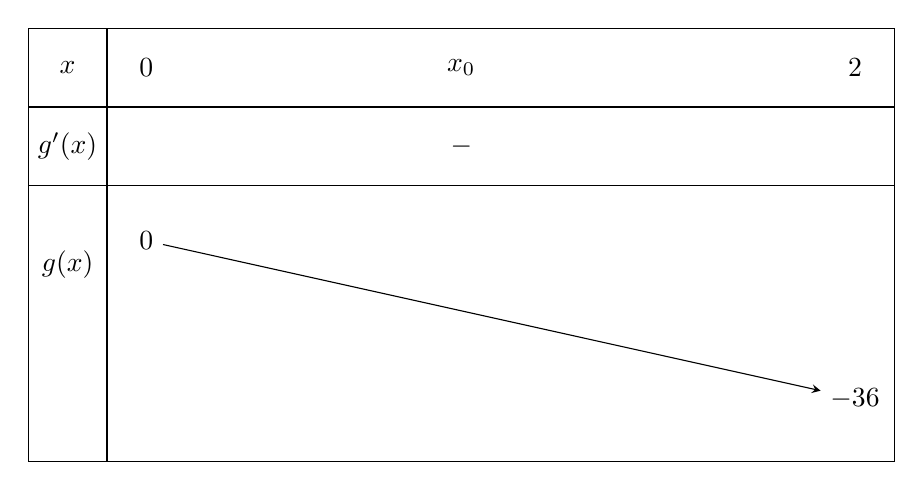
\begin{tikzpicture}
					\foreach \x/\texn in {-4/x,
						-3/0,  1/x_0, 6/2} \path
					(\x,3.5)node{$\texn$};
					\foreach \x/\texn in
					{-4/g’(x),1/-} \path
					(\x,2.5)node{$\texn$};
					\foreach \x/\y/\texn in {-4/1/g(x),
						-3/1.3/0,6/-0.7/-36}
					\path (\x,\y) node(\x){$\texn$};
					\draw[-stealth] (-3)--(6);
					\draw
					(-4.5,4)--(6.5,4) (-3.5,4)--(-3.5,-1.5)
					(-4.5,3)--(6.5,3) (-4.5,2)--(6.5,2)
					(-4.5,4) rectangle (6.5,-1.5);
					\end{tikzpicture}	
			\end{center}
			Từ bảng biến thiên ta có $g(x)\in [-36;0]$, $\forall x\in [0;2]$.\\
			\begin{itemize}
			\item \textbf{Trường hợp 1} $m>0\Rightarrow $ phương trình $(1)$ vô nghiệm $\Leftrightarrow$ phương trình $y'=0$  vô nghiệm.\\
			Dễ thấy $y(0)=-m<y(2)=4-\dfrac{m}{3}$ khi $m>0$.\\
			Khi đó $\max \limits_{[0;2]}y=y(2)=4-\dfrac{m}{3}=5\Leftrightarrow m=-3$  loại do $m>0$.
			\item \textbf{Trường hợp 2} $m<-36$  phương trình $(1)$ vô nghiệm $\Leftrightarrow$ phương trình $ y'=0$  vô nghiệm.\\
			Dễ thấy $y(0)=-m>y(2)=4-\dfrac{m}{3}$ khi $m<-36$.\\
			Khi đó  $\max \limits_{[0;2]}y=y(0)=-m=5\Leftrightarrow m=-5$  loại do $m<-36$.
			\item \textbf{Trường hợp 3} $m\in [-36;0]\Rightarrow $   phương trình $y'=0$ có nghiệm duy nhất (giả sử $x=x_0$ ).\\
			Trên $[0;2] $  ta có bảng biến thiên
			\begin{center}
			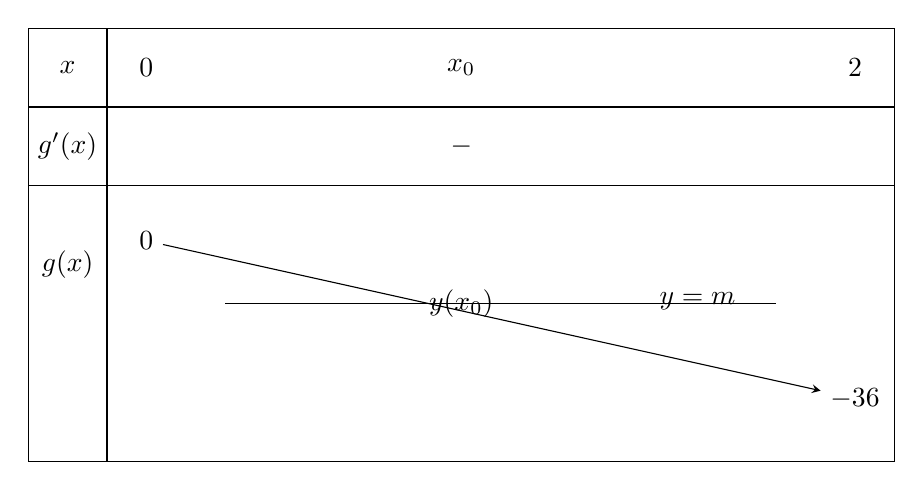
\begin{tikzpicture}
				\foreach \x/\texn in {-4/x,
					-3/0,  1/x_0, 6/2} \path
				(\x,3.5)node{$\texn$};
				\foreach \x/\texn in
				{-4/g’(x),1/-} \path
				(\x,2.5)node{$\texn$};
				\foreach \x/\y/\texn in {-4/1/g(x),
					-3/1.3/0,1/0.5/y(x_0),6/-0.7/-36}
				\path (\x,\y) node(\x){$\texn$};
				\draw[-stealth] (-3)--(6);
				\draw
				(-4.5,4)--(6.5,4) (-3.5,4)--(-3.5,-1.5)
				(-4.5,3)--(6.5,3) (-4.5,2)--(6.5,2)(-2,0.5)--(5,0.5)
				(-4.5,4) rectangle (6.5,-1.5);
				\node[above] at (4,0.3){\text{$y=m$}};
				\end{tikzpicture}	
			\end{center}
			
			Nhìn vào bảng biến thiên ta có:
		\begin{itemize}
			\item $x=x_0$ Khi đó $g(x)=m\Leftrightarrow -\left(2x^3+4x^2+2x\right)=m\Leftrightarrow 2x^3+4x^2+2x+m=0\Leftrightarrow y'=0$.
			\item $x\in (0;x_0)$ Khi đó $g(x)>m\Leftrightarrow -\left(2x^3+4x^2+2x\right)>m\Leftrightarrow 2x^3+4x^2+2x+m<0\Leftrightarrow y'<0$.
			\item $x\in (x_0;0)$ Khi đó $g(x)<m\Leftrightarrow -\left(2x^3+4x^2+2x\right)<m\Leftrightarrow 2x^3+4x^2+2x+m>0\Leftrightarrow y'>0$.
		\end{itemize}
			Ta có bảng biến thiên sau
			\begin{center}
				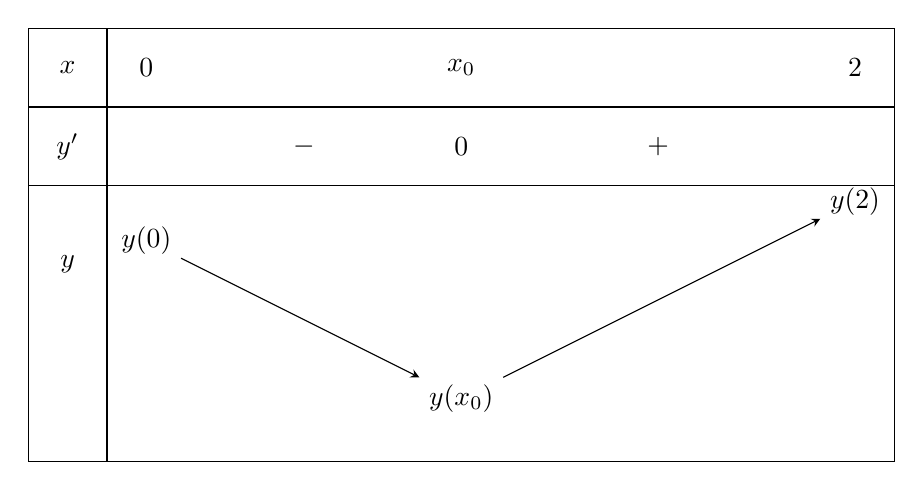
\begin{tikzpicture}
					\foreach \x/\texn in {-4/x,
						-3/0,  1/x_0, 6/2} \path
					(\x,3.5)node{$\texn$};
					\foreach \x/\texn in
					{-4/y’,-1/-,1/0,3.5/+} \path
					(\x,2.5)node{$\texn$};
					\foreach \x/\y/\texn in {-4/1/y,
						-3/1.3/y(0),1/-0.7/y(x_0),6/1.8/y(2)}
					\path (\x,\y) node(\x){$\texn$};
					\draw[-stealth] (-3)--(1);
					\draw[-stealth](1)--(6);
							\draw
					(-4.5,4)--(6.5,4) (-3.5,4)--(-3.5,-1.5)
					(-4.5,3)--(6.5,3) (-4.5,2)--(6.5,2)
					(-4.5,4) rectangle (6.5,-1.5);
				\end{tikzpicture}
			\end{center} 
			
			Từ bảng biến thiên ta thấy $\max \limits_{[0;2]}y\in \{y(2);y(0)\}$.\\
			Nếu $m\in [-36;-6]\Rightarrow y(0)\geq y(2)\Rightarrow \max \limits_{[0;2]}y=y(0)=-m=5\Leftrightarrow m=-5$ (loại).\\
			Nếu $m\in [-6;0]\Rightarrow y(0)<y(2)\Rightarrow \max \limits_{[0;2]}y=y(2)=4-\dfrac{m}{3}=5\Leftrightarrow m=-3$ (nhận).\\
			Vậy $m=-3$  thỏa mãn bài toán.
		\end{itemize}
	
	}
\end{ex}
%%%%-Câu 25
\begin{ex}%[2D1K3-2]
	Câu 25.	Cho hàm số $y=\left(x^3-3x+m\right)^2$. Tổng tất cả các giá trị của tham số $m$ sao cho giá trị nhỏ nhất của hàm số trên đoạn $[-1;1]$  bằng $1$ là
	\choice 
	{$1$}
	{$-4$}
	{\True $0$}
	{$4$}
	\loigiai{
	$\mathscr{D}=\mathbb{R}$
Đặt $t=x^3-3x$, $x\in [-1;1]\Rightarrow tg\in [-2;2]$.\\
Khi đó ta có hàm số $f(t)=\left(t+m\right)^2$\\
 $f'(t)=2\left(t+m\right)$\\
 $f'(t)=0\Leftrightarrow t=-m$.\\
\begin{itemize}
	\item \textbf{Trường hợp 1} $-2<-m<2\Leftrightarrow -2<m<2$.
	\begin{center}
		\begin{tikzpicture}
			\foreach \x/\texn in {-4/t,
				-3/,-1/-2, 2/-m, 5/2, 7/+\infty} \path
			(\x,3.5)node{$\texn$};
			\foreach \x/\texn in
			{-4/f’(t),0.5/-,2/0,3.5/+} \path
			(\x,2.5)node{$\texn$};
			\foreach \x/\y/\texn in {-4/1/f(t),
				-1/1.8/,2/-0.5/f(-m),5/1.8/,}
			\path (\x,\y) node(\x){$\texn$};
			\draw[-stealth] (-1)--(2);
			\draw[-stealth](2)--(5);
			\draw
			(-4.5,4)--(7.5,4) (-3.5,4)--(-3.5,-1)
			(-4.5,3)--(7.5,3) (-4.5,2)--(7.5,2)
			(-4.5,4) rectangle (7.5,-1);
			\begin{scope}
				\fill[pattern=north east lines] (-3,4)--(-1,4)--(-1,-1)--(-3,-1)--cycle;
				%\draw (-1,-3)--(1.5,2) node [pos=0.45, above, sloped] {};
				\fill[pattern=north east lines] (5,4)--(7,4)--(7,-1)--(5,-1)--cycle;
			\end{scope}
		\end{tikzpicture}
	\end{center}	
	Từ bảng biến thiên ta thấy $\min \limits_{[-2;2]}f(t)=f(-m)=0$ không thoả mãn yêu cầu.
	\item \textbf{Trường hợp 2} $-m\leq -2\Leftrightarrow m\geq 2$.
	\begin{center}
		\begin{tikzpicture}
			\foreach \x/\texn in {-4/t,
				-3/,-1/-m, 2/-2, 5/2, 7/+\infty} \path
			(\x,3.5)node{$\texn$};
			\foreach \x/\texn in
			{-4/f’(t),-2/-,-1/0,3.5/+} \path
			(\x,2.5)node{$\texn$};
			\foreach \x/\y/\texn in {-4/1/f(t),
				2/-0.7/f(-2),5/1.7/f(2),}
			\path (\x,\y) node(\x){$\texn$};
			\draw[-stealth](2)--(5);
			\draw
			(-4.5,4)--(7.5,4) (-3.5,4)--(-3.5,-1)
			(-4.5,3)--(7.5,3) (-4.5,2)--(7.5,2)
			(-4.5,4) rectangle (7.5,-1);
			\begin{scope}
				\fill[pattern=north east lines] (-3,4)--(2,4)--(2,-1)--(-3,-1)--cycle;
				%\draw (-1,-3)--(1.5,2) node [pos=0.45, above, sloped] {};
				\fill[pattern=north east lines] (5,4)--(7,4)--(7,-1)--(5,-1)--cycle;
			\end{scope}
		\end{tikzpicture}
	\end{center} 
	Từ bảng biến thiên ta thấy $\min \limits_{[-2;2]}f(t)=f(-2)=\left(m-2\right)^2$.\\
	 Theo yêu cầu của bài toán $\left(m-2\right)^2=1\Leftrightarrow\hoac{&m=3\\&m=1}$.\\
	  Do $m\geq 2$ nên $m=3$.
	\item \textbf{Trường hợp 3} $-m\geq 2\Leftrightarrow m\leq -2$.
	\begin{center}
		\begin{tikzpicture}
		\foreach \x/\texn in {-4/t,
			-3/, 2/-2, 5/2, 7/-m,9/+\infty} \path
		(\x,3.5)node{$\texn$};
		\foreach \x/\texn in
		{-4/f’(t),3.5/-,7/0,8/+} \path
		(\x,2.5)node{$\texn$};
		\foreach \x/\y/\texn in {-4/1/f(t),
			2/1.7/f(2),5/-0.7/f(2),}
		\path (\x,\y) node(\x){$\texn$};
		\draw[-stealth] (2)--(5);
		\draw
		(-4.5,4)--(9.5,4) (-3.5,4)--(-3.5,-1)
		(-4.5,3)--(9.5,3) (-4.5,2)--(9.5,2)
		(-4.5,4) rectangle (9.5,-1);
		\begin{scope}
			\fill[pattern=north east lines] (-3,4)--(2,4)--(2,-1)--(-3,-1)--cycle;
			%\draw (-1,-3)--(1.5,2) node [pos=0.45, above, sloped] {};
			\fill[pattern=north east lines] (5,4)--(9.5,4)--(9.5,-1)--(5,-1)--cycle;
		\end{scope}
	\end{tikzpicture}	
	\end{center}
	 Từ bảng biến thiên ta thấy $\min \limits_{[-2;2]}f(t)=f(2)=\left(m+2\right)^2$.\\
	 Theo yêu cầu của bài toán $\left(m+2\right)^2=1\Leftrightarrow \hoac{&m=-3\\&m=-1}$.\\
	 Do $m\leq -2$ nên $m=-3$.\\
	  Vậy tổng các giá trị của $m$ thoả mãn yêu cầu là $3+(-3)=0$.
\end{itemize}}
\end{ex}
%%%%-Câu 26
\begin{ex}%[2D1K3-2]
	Tìm tất cả các giá trị của $m>0$ để giá trị nhỏ nhất của hàm số $y=x^3-3x+1$  trên đoạn $[m+1;m+2]$  luôn bé hơn  $3$.
	\choice
	{$m\in (0;2)$}
	{$m\in (0;1)$}
	{$m\in (1;+\infty)$}
	{$m\in (0;+\infty)$}
	\loigiai{
	Ta có $y'=3x^2-3$, $y'=0\Leftrightarrow x=\pm 1$  do đó $y_{CT}=y(1)=-1$ và  $y_{\text{CĐ}}=y(-1)=3$.\\
	Thấy ngay với $m>0$  thì trên đoạn $[m+1;m+2]$  hàm số luôn đồng biến.\\
	Vậy GTNN của hàm số đã cho trên đoạn $[m+1;m+2]$ là $y(m+1)=\left(m+1\right)^3-3\left(m+1\right)+1$.\\
	GTNN luôn bé hơn $3\Leftrightarrow \left(m+1\right)^2-3\left(m+1\right)-2<0\Leftrightarrow \heva{&m+1<2\\&m+1\neq -1}\Leftrightarrow \heva{&m<1\\&m\neq -2.}$ \\
	Kết hợp điều kiện  $m>0$ ta được $m\in (0;1)$.
}
\end{ex}
%%%%-Câu 27
\begin{ex}%[2D1K3-2]
	Biết rằng giá trị nhỏ nhất của hàm số $y=mx+\dfrac{36}{x+1}$  trên $[0;3]$   bằng $20$. Mệnh đề nào sau đây đúng?
	\choice 
	{$0<m\leq 2$}
	{$4<m\leq 8$}
	{\True $2<m\leq 4$}
	{$m>8$}
	\loigiai{
$y=mx+\dfrac{36}{x+1}\Rightarrow y'=\dfrac{36}{(x+1)^2}$
\begin{itemize}
	\item \textbf{Trường hợp 1} $m=0$, ta có $y'\dfrac{36}{(x+1)^2}<0\, \forall x\neq -1$. Khi đó $\min \limits_{[0;3]}y=y(3)=9$ (loại).
	\item \textbf{Trường hợp 2} $m\neq 0$
	\begin{itemize}
		\item Nếu $m<0$, ta có $y'<0$, $\forall x\neq -1$. Khi đó $\min \limits_{[0;3]}y=y(3)\Leftrightarrow 20=3m+9\Leftrightarrow m=\dfrac{11}{3}$ (loại).
		\item Nếu $m>0$, ta có $y'=0\Leftrightarrow m-\dfrac{36}{(x+1)^2}=0\Leftrightarrow (x+1)^2=\dfrac{36}{m}\Leftrightarrow \hoac{&x\dfrac{6}{\sqrt{m}}-1\\&x=-\dfrac{6}{\sqrt{m}}-1 \, \text{(loại).}}$
		\item $0<\dfrac{6}{\sqrt{m}}-1\leq 3\Leftrightarrow \dfrac{4}{9}<m\leq 36$, $\min \limits_{[0;3]}y=y\left(\dfrac{6}{\sqrt{m}}-1\right)=12\sqrt{m}-m=20\Leftrightarrow \hoac{&m=4\\&m=100\, \text{(loại)}}$.
		\item $\dfrac{6}{\sqrt{m}}-1>3\Leftrightarrow m<\dfrac{9}{4}$, $\min \limits_{[0;3]}y=y(3)\Leftrightarrow 20=3m+9\Leftrightarrow m=\dfrac{11}{3}$ (loại).
	\end{itemize}
\end{itemize}	
}
\end{ex}
%%%%-Câu 28
\begin{ex}%[2D1K3-2]
	Cho hàm số $y=x^3-3mx^2+3\left(m^2-1\right)x+2020$. Có tất cả bao nhiêu giá trị nguyên của $m$ sao cho hàm số có giá trị nhỏ nhất trên khoảng $(0;+\infty)$?
	\choice 
	{$2$}
	{$1$}
	{Vô số}
	{\True $3$} 
	\loigiai{
	Ta có $y'=3x^2-6mx+3\left(m^2-1\right)=0\Leftrightarrow \hoac{&x_1=m-1\\&x_2=m+1.}$  .
	Để hàm số có giá trị nhỏ nhất trên khoảng $(0;+\infty)$ thì $x_1\leq 0<x_2$ hoặc $0<x_1<x_2$.
	\begin{itemize}
		\item \textbf{Trường hợp 1} $x_1\leq 0<x_2\Leftrightarrow m-1\leq 0<m+1\Leftrightarrow -1<m\leq 1$.\\
		Do $m\in \mathbb{Z}\Rightarrow m\in \{0;1\}$.\\
		 Bảng biến thiên của hàm số 
		 \begin{center}
		 	
\begin{tikzpicture}
		 		\tkzTab
		 		[lgt=2,espcl=4] % tùy chọn
		 		{$x$/1, $y’(x)$/0.8, $y(x)$/2} % cột đầu tiên
		 		{$0$,$m+1$,$+\infty$} % hàng 1 cột 2
		 		{,-,0,+,} % hàng 2 cột 2
		 		{+/,-/, +/ } % hàng 3 cột 2
		 	\end{tikzpicture}
		 \end{center} 	
		\item \textbf{Trường hợp 2} $0<x_1<x_2$. 
		Bảng biến thiên của hàm số
		\begin{center}
			
\begin{tikzpicture}
				\tkzTab
				[lgt=2,espcl=4] % tùy chọn
				{$x$/1, $y’(x)$/0.8, $y(x)$/2} % cột đầu tiên
				{$0y$,$m-1$,$m+1$,$+\infty$} % hàng 1 cột 2
				{,+,0,-,0,+,} % hàng 2 cột 2
				{-/ , +/, -/, +/} % hàng 3 cột 2
			\end{tikzpicture}
		\end{center}
		Hàm số có giá trị nhỏ nhất trên khoảng  $(0;+\infty)$ khi và chỉ khi 
		$\heva{&m-1>0\\&y(m+1)\leq y(0)}\Leftrightarrow \heva{&m>1\\&(m+1)^3-3m(m+1)^2+3(m^2-1)(m+1)+2020\leq2020}\Leftrightarrow \heva{&m>1\\&(m+1)^2(m-2)\leq 0}\Leftrightarrow \heva{&m>1\\&\hoac{&m\leq 2\\&m=-1}}\Leftrightarrow 1<m\leq 2.$\\
		 Do $m\in \mathbb{Z}\Rightarrow m=2$.
	\end{itemize}
	Vậy $m\in \{0;1;2\}$.
}
\end{ex}
%%%%-Câu 29
\begin{ex}
	Cho hàm số  $f(x)=m\sqrt{x-1}$ ( $m$ là tham số thực khác $0$). Gọi $m_1$, $m_2$ là hai giá trị của $m$ thoả mãn $\min \limits_{[2;5]}f(x)+\max \limits_{[2;5]}f(x)=m^2-10$. Giá trị của $m_1+m_2$ bằng
	\choice 
	{\True $3$}
	{$5$}
	{$10$}
	{$2$} 
	\loigiai{
	Ta có $f'(x)=m\dfrac{1}{2\sqrt{x-1}}$;
	Do $m\neq 0$  nên $f'(x)$  khác $0$ và có dấu không thay đổi với $\forall x\in (1;+\infty)$.  
	Nếu $m>0$  thì $f'(x)>0 $, $\forall x\in [2;5]$.\\
	Do đó $\min \limits_{[2;5]}f(x)=f(2)=m$; $\max \limits_{[2;5]}f(x)=f(5)=2m$.\\ 
	$\min \limits_{[2;5]}f(x)+\max \limits_{[2;5]}f(x)=m^2-10\Leftrightarrow m+2m=m^2-10\Leftrightarrow m^2-3x-10=0\hoac{&m_1=-2\\&m_2=5.}$
	Do  $m>0$ nên nhận $m_2=5$.\\  
	Nếu $m<0$  thì $f'(x)<0$, $\forall x\in [2;5]$.\\
	 Do đó  $\min \limits_{[2;5]}f(x)=f(5)=2m$; $\max \limits_{[2;5]}f(x)=f(2)=m$.\\ 
	$\min \limits_{[2;5]}f(x)+\max \limits_{[2;5]}f(x)=m^2-10\Leftrightarrow 2m+m=m^2-10\Leftrightarrow m^2-3x-10=0\hoac{&m_1=-2\\&m_2=5.}$
	Do  $m<0$ nên nhận $m_2=-2$.\\  
Vậy $m_1+m_2=3.$
}
\end{ex}
%%%%-Câu 30
\begin{ex}%[2D1K3-2]
	 Cho hàm số $y=\dfrac{m\sin x+1}{\cos x+2}$  có bao nhiêu giá trị nguyên của tham số $m$ thuộc đoạn $[-5;5]$ để giá trị nhỏ nhất của $y$ nhỏ hơn $-1$.
	 \choice 
	 {$4$}
	 {$2$}
	 {\True $6$}
	 {$8$}
	 \loigiai{Điều kiện $\cos x+2\neq 0$ luôn đúng $\forall x\in \mathbb{R}$.\\ 
	 	$y=\dfrac{m\sin x+1}{\cos x+2}\Leftrightarrow y\left(\cos x+2\right)=m\sin x+1$
	 	(do $\cos x+1\neq 0$  luôn đúng $\forall x\in \mathbb{R}$).\\
	 	$\Leftrightarrow m\sin x-y\cos x=2y-1 \, (*)$.
	 	Phương trình (*) có nghiệm $\Leftrightarrow m^2+y^2\geq \left(2y-1\right)^2\Leftrightarrow 3y^2-4y+1-m^2\leq 0\Leftrightarrow \dfrac{2-\sqrt{1+3m^2}}{3}\leq yh\leq \dfrac{2+\sqrt{1+3m^2}}{3}$.\\
	 	Vậy $\min \limits_{\mathbb{R}}y\dfrac{2-\sqrt{1+3m^2}}{3}$.\\
	 	$\min \limits_{\mathbb{R}}y<-1\Leftrightarrow \dfrac{2-\sqrt{1+3m^2}}{3}<-1\Leftrightarrow \sqrt{1+3m^2}>5\Leftrightarrow m^2-8>0\Leftrightarrow \hoac{&m>2\sqrt{2}\\&m<-2\sqrt{2}.}$.
	 	Mà $m\in \mathbb{Z}$,$m\in [-5;5]$  nên $m\in \{-5;-4;-3;3;4;5\}$.\\
	 	 Vậy có tất cả $6$ giá trị của $m$ thoả đề bài.
	 	
	 }
\end{ex}
%%%%-Câu 31
\begin{ex}%[2D1K3-2]
	Gọi $S$  là tập hợp tất cả các giá trị thực của tham số $m$  sao cho giá trị nhỏ nhất của hàm số $f(x)=\dfrac{34}{\sqrt{\left(x^3-3x+2m\right)^2+1}}$   trên đoạn $[0;3]$  bằng $2$. Tổng tất cả các phần tử của $S$  bằng
	\choice
	{$8$}
	{\True $-8$}
	{$-6$}
	{$-1$}
	\loigiai{ Ta có $\sqrt{\left(x^3-3x+2m\right)^2}=\mid x^3-3x+2\mid$.\\
		Nhận thấy $\min \limits_{[0;3]}f(x)=2\Leftrightarrow \max \limits_{[0;3]}f(x)=16\, (1)$.\\
		Xét hàm số $g(x)=x^3-3x+2m$  trên $[0;3]$, ta có:
		\begin{itemize}
			\item $g'(x)=3x^2-3=0\Leftrightarrow \hoac{&x=1\in (0;3)\\&x=-1\notin (0;3)}$.
			\item $g(0)=2m$, $g(1)=2m-2$, $g(3)=2m+18$.
		\end{itemize}	
		Do đó $2m-2\leq g(x)\leq 2m+18$, $\forall x\in [0;3]$ tức $\max \limits_{[0;3]}\mid x^3-3x+2m\mid =\max \limits_{[0;3]}\left\{\mid 2m-2\mid ; \mid 2m+18\mid \right\}$.\\
		Từ đây ta có $(1)\Leftrightarrow \max \limits_{[0;3]}\left\{\mid 2m-2\mid ; \mid 2m+18\mid \right\}=16\Leftrightarrow \hoac{&\heva{&\mid 2m+18 \mid >\mid 2m-2 \mid \\& \mid 2m+18\mid =16}\\&\heva{&\mid 2m+18 \mid \leq \mid 2m-2 \mid \\& \mid 2m-2\mid =16}}\Leftrightarrow \hoac{&m=-1\\&m=-7}$.\\ 
	Suy ra $S=\{-7;-1\}$. Vậy  tổng các phần tử của $S$ là $-8$.		
	}
\end{ex}
%%%%-Câu 32
\begin{ex}%[2D1K3-2]
	Cho hàm số $y=\left(x^3-3x+m+1\right)^2$. Tổng tất cả các giá trị của tham số $m$ sao cho giá trị nhỏ nhất của hàm số trên đoạn $[-1;1]$ bằng $1$ là
	\choice 
	{$-2$}
	{$4$}
	{$-4$}
	{$0$}
	\loigiai{
	Đặt $y=f(x)=\left(x^3-3x+m+1\right)^2$  là hàm số xác định và liên tục trên đoạn $[-1;1]$.\\
	Ta có $y'=f'(x)=2\left(x^3-3x+m+1\right)\cdot \left(3x^2-2\right)$.\\
	$f'(x)=0\Leftrightarrow \hoac{&x=\pm 1\\&m=-x^3+3x-1=g(x).}$.\\
	Ta khảo sát hàm số $g(x)$  trên đoạn $[-1;1]$.\\
	Bảng biến thiên của  $g(x)$.
	\begin{center}
		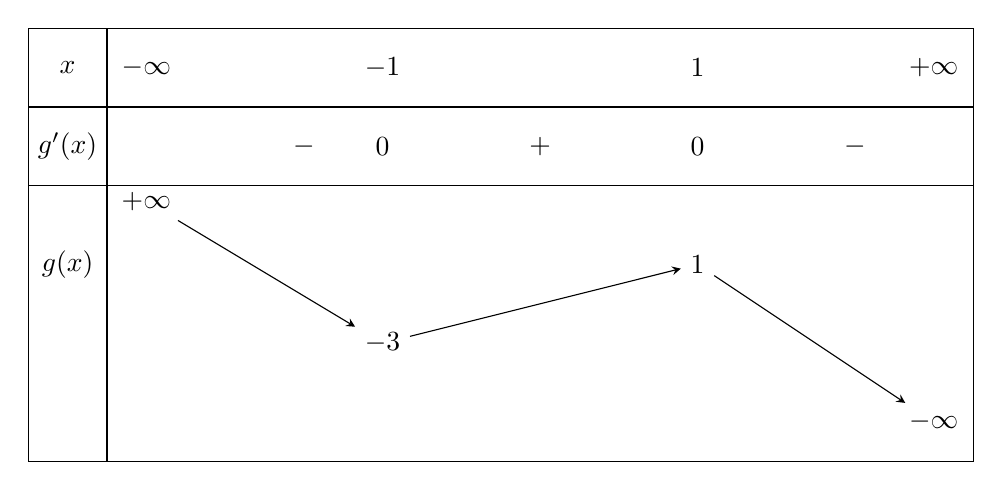
\begin{tikzpicture}
			\foreach \x/\texn in {-4/x,
				-3/-\infty,0/-1,  4/1, 7/+\infty} \path
			(\x,3.5)node{$\texn$};
			\foreach \x/\texn in
			{-4/g’(x),-1/-,0/0,2/+,4/0,6/-} \path
			(\x,2.5)node{$\texn$};
			\foreach \x/\y/\texn in {-4/1/g(x),
				-3/1.8/+\infty,0/0/-3,4/1/1,7/-1/-\infty}
			\path (\x,\y) node(\x){$\texn$};
			\draw[-stealth] (-3)--(0);
			\draw[-stealth](0)--(4);
			\draw[-stealth] (4)--(7);
			\draw
			(-4.5,4)--(7.5,4) (-3.5,4)--(-3.5,-1.5)
			(-4.5,3)--(7.5,3) (-4.5,2)--(7.5,2)
			(-4.5,4) rectangle (7.5,-1.5);
		\end{tikzpicture}
	\end{center} 	
	Nếu $m\in [-3;1]$  thì luôn tồn tại $x_0\in [-1;1]$  sao cho $m=g(x_0)$  hay $f(x_0)=0$. \\
	Suy ra $\min \limits_{[-1;1]}y=0$,  tức là không tồn tại $m$  thỏa mãn yêu cầu bài toán.\\
	Nếu $m\notin [-3;1]$  thì $f'(x)=0\Leftrightarrow x=\pm 1\in [-1;1]$.\\
	Ta có $\min \limits_{[-1;1]}f(x)=\min \left\{f(1);f(-1)\right\}=\min \left\{\left(m-1\right)^2;\left(m+3\right)^2\right\}$.
	\begin{itemize}
		\item \textbf{Trường hợp 1} $m>1$ tức là $m+3>m-1>0$ suy ra $\min \limits_{[-1;1]}f(x)=(m-1)^2=1\Leftrightarrow \hoac{&m=0 \, \text{(loại)}\\&m=2 \, \text{(nhận)}.}$
		\item \textbf{Trường hợp 2} $m<-3$ tức là $m-1<m+3<0$ suy ra $\min \limits_{[-1;1]}f(x)=(m+3)^2=1\Leftrightarrow \hoac{&m=-2 \, \text{(loại)}\\&m=-4 \, \text{(nhận)}.}$
	\end{itemize}	
	Vậy có hai giá trị của  $m$ thỏa mãn yêu cầu bài toán, do đó tổng tất cả các giá trị của $m$  là $-2$.
}
\end{ex}
%%%%-Câu 33
\begin{ex}%[2D1K3-2]
	Cho hàm số $y=f(x)=m^2\left(\sqrt{2+x}+\sqrt{2-x}\right)+4\sqrt{4-x^2}+m+1$. Tính tổng tất cả các giá trị của $m$ để hàm số $y=f(x)$ có giá trị nhỏ nhất bằng $4$.
	\choice
	{$-\dfrac{7}{2}$}
	{$\dfrac{5}{2}$}
	{\True $-\dfrac{1}{2}$}
	{$\dfrac{1}{2}$}
	\loigiai{Tập xác định $\mathscr{D}=[-2;2]$.\\
		Đặt $t=\sqrt{2+x}+\sqrt{2-x}$; $t\in [2;2\sqrt{2}]$.\\
		$t^2=4+2\sqrt{4-x^2}\Leftrightarrow 2\sqrt{4-x^2}=t^2-4$.\\
		$\Rightarrow y=g(t)=m^2t+2(t^2-4)+m+1=2t^2+m^2t+m-7$
		với $t\in [2;2\sqrt{2}]$.\\
		Ta có $g'(t)=4t+m^2$.\\
		 $g'(t)=0\Leftrightarrow t=\dfrac{-m^2}{4}<0$, $\forall m\in \mathbb{R}\Rightarrow g(t)$ 
		đồng biến trên $[2;2\sqrt{2}]\Rightarrow \min \limits_{[2;2\sqrt{2}]}g(t)=g(2)=4$.\\
		Mà  $g(2)=2m^2+m+1\Leftrightarrow 2m^2+m+1=4\Leftrightarrow \hoac{&m=1\\&m=-\dfrac{3}{2}.}$ \\
		Tổng các giá trị của $m$  thỏa mãn ycbt là $S=1+\left(-\dfrac{3}{2}\right)=-\dfrac{1}{2}$.
		
	}
\end{ex}
%%%%-Câu 34
\begin{ex}%[2D1K3-2]
	Cho hàm số $f(x)=\dfrac{2x-m}{x+1}$  với $m\neq -2$. Mệnh đề nào dưới đây sai?
	\choice 
	{$\max \limits_{[1;3]}f(x)=\max \left\{\dfrac{2-m}{2};\dfrac{6-m}{4}\right\}$}
	{\True $\max \limits_{[1;3]}f(x)=\dfrac{6-m}{2}$ khi $m<-2$}
	{$\min \limits_{[1;3]}f(x)=\max \left\{\dfrac{2-m}{2};\dfrac{6-m}{4}\right\}$}
	{\True $\min \limits_{[1;3]}f(x)=\dfrac{2-m}{2}$ khi $m>-2$}
	\loigiai{
	Tập xác định $\mathscr{D}=\mathbb{R}\setminus\{-1\}$.\\
	Ta có $f'(x)=\dfrac{2+m}{(x+1)^2}$  suy đạo hàm không đổi dấu $x\in [1;3]$  suy ra $\max \limits_{[1;3]}f(x)=\max \left\{f(1);f(3)\right\}=\max \left\{\dfrac{2-m}{2};\dfrac{6-m}{4}\right\}$;\\
	$\min \limits_{[1;3]}f(x)=\max \left\{f(1);f(3)\right\}=\min \left\{\dfrac{2-m}{2};\dfrac{6-m}{4}\right\}$.\\
	Xét với $m<-2\Rightarrow f'(x)<0\, \forall x\in [1;3]$.\\
	 Vậy $\forall x\in [1;3]\Rightarrow f(x)\leq f(1)=\dfrac{2-m}{2}\Rightarrow \max \limits_{[1;3]}f(x)=\dfrac{2-m}{2}$.\\
	Xét với $m>-2\Rightarrow f'(x)>0\, \forall x\in [1;3]$. Vậy $\forall x\in [1;3]\Rightarrow f(x)\geq f(1)=\dfrac{2-m}{2}\Rightarrow \min \limits_{[1;3]}f(x)=\dfrac{2-m}{2}$.
}
\end{ex}
%%%%-Câu 35
\begin{ex}%[2D1K3-2]
	Có bao nhiêu số nguyên $m$  thuộc đoạn $[-20;20]$  để giá trị lớn nhất của hàm số $y=\dfrac{x+m+6}{x-m}$  trên đoạn $[1;3]$  là số dương?
	\choice 
	{\True $9$}
	{$8$}
	{$11$}
	{$10$}
	\loigiai{
	Tập xác định $\mathscr{D}=\mathbb{R}\setminus\{m\}$.\\ 
	Để hàm số có giá trị lớn nhất trên $[1;3]$  thì $m\notin [1;3]$.\\  
	$y'=\dfrac{-2m-6}{(x-m)^2}.$\\
	\begin{itemize}
		\item \textbf{Trường hợp 1} $-2m-6>0\Leftrightarrow m<-3$.\\
		 Khi đó  $\max \limits_{[1;3]}y=y(3)=\dfrac{m+9}{3-m}$.\\
		 Để giá trị lớn nhất trên đoạn $[1;3]$ là số dương thì $\dfrac{m+9}{3-m}>0\Leftrightarrow m+9>0\Leftrightarrow m>-9$.\\  
		 Vậy các số nguyên $m$  thỏa là $-8;-7-6;-5;-4$.  
		\item \textbf{Trường hợp 2} $-2m-6<0\Leftrightarrow m>-3$.
		$\max \limits_{[1;3]}y=y(1)=\dfrac{m+7}{1-m}$.\\
		Để giá trị lớn nhất trên đoạn $[1;3]$ là số dương thì $\dfrac{m+7}{1-m}>0\Leftrightarrow 1-m>0\Leftrightarrow m<1$.\\  
		Vậy các số nguyên $m$  thỏa là $-2;-1;0$.   
		\item \textbf{Trường hợp 3} $-2m-6=0\Leftrightarrow m=-3$.
		Khi đó $y=1$. Nên $\max \limits_{[1;3]}y=1$.\\  
		Vậy $m=-3$  thỏa.
	\end{itemize}
Vậy có $9$ số nguyên   thỏa mãn yêu cầu bài toán.
}
\end{ex}
%%%%-Câu 36
\begin{ex}
	Cho hàm số $f(x)=(m-1)x^4-2mx^2+1$  với $m$  là tham số thực. Nếu $\min \limits_{[0;3]}f(x)=f(2)$  thì $\max \limits_{[0;3]}f(x)$  bằng
	\choice
	{$-\dfrac{13}{3}$}
	{\True $4$}
	{$-\dfrac{14}{3}$}
	{$1$} 
	\loigiai{
	 Ta có $f'(x)=4(m-1)x^3-4mx=4x\left[(m-1)x^2-m\right]$\\
 $f'(x)=0\Leftrightarrow \hoac{&x=0\\&x^2=\dfrac{m}{m-1}}$ ($m=1$ không thoả yêu cầu bài toán)\\
Vì $\min \limits_{[0;3]}f(x)=f(2)\Rightarrow x=2$ là nghiệm của $f'(x)=0$\\
 $\Rightarrow \dfrac{m}{m-1}=4\Rightarrow m=4m-4\Rightarrow m=\dfrac{4}{3}$.\\
  $\Rightarrow f(x)=\dfrac{1}{3}x^4-\dfrac{8}{3}x^2+1$\\
  $f(0)=1$, $f(3)=\dfrac{81}{3}-\dfrac{72}{3}+\dfrac{3}{3}=\dfrac{12}{3}=4$.\\
   $\max \limits_{[0;3]f(x)=4}$. 
}
\end{ex}
%%%%-Câu 37
\begin{ex}%[2D1K3-2]
	 Cho hàm số $f(x)=mx^4+2(m-1)x^2$ với $m$ là tham số thực. Nếu $\min \limits_{[0;2]}f(x)=f(1)$ thì $\max \limits_{[0;2]}f(x)$  bằng
	 \choice 
	 {$2$}
	 {$-1$}
	 {\True $4$}
	 {$0$}
	 \loigiai{
	 $f'(x)=4mx^3+4(m-1)x$\\
 Do $f(x)$ là hàm đa thức và $\min \limits_{[0;2]}f(x)=f(1)\Rightarrow f'(1)=0\Leftrightarrow 4m+4(m-1)=0\Leftrightarrow m=\dfrac{1}{2}$.\\
 Thay $m=\dfrac{1}{2}$ vào hàm số ban đầu ta được\\
 $y=\dfrac{1}{2}x^4+2\left(\dfrac{1}{2}-1\right)x^2=\dfrac{1}{2}x^4-x^2\Rightarrow y'=2x^3-2x=2x\left(x-1\right)\left(x+1\right)$.\\
 Ta có bảng biến thiên
 \begin{center}
 	 \begin{tikzpicture}
 		\foreach \x/\texn in {-4/x,
 			-3/-\infty,-1/-1,1/0, 3/1, 5/2, 7/+\infty} \path
 		(\x,3.5)node{$\texn$};
 		\foreach \x/\texn in
 		{-4/g’(x),-2/-,-1/0,0/+,1/0,2/-,3/0,4/+,6/+} \path
 		(\x,2.5)node{$\texn$};
 		\foreach \x/\y/\texn in {-4/1/g(x),
 			-3/1.8/+\infty,-1/-1/-\dfrac{1}{2},1/-0.5/0,3/-1/-\dfrac{1}{2} , 5/0.5/4,7/1.8/+\infty}
 		\path (\x,\y) node(\x){$\texn$};
 		\draw[-stealth] (-3)--(-1);
 		\draw[-stealth](-1)--(1);
 		\draw[-stealth] (1)--(3);
 		\draw[-stealth](3)--(5);
 		\draw[-stealth] (5)--(7);
 		\draw
 		(-4.5,4)--(7.5,4) (-3.5,4)--(-3.5,-1.5)
 		(-4.5,3)--(7.5,3) (-4.5,2)--(7.5,2)
 		(-4.5,4) rectangle (7.5,-1.5);
 	\end{tikzpicture}
 \end{center} 	
Vậy với $m=\dfrac{1}{2}$ thì $\min \limits_{[0;2]}f(x)=f(1)$ (thoả mãn).\\
Dựa vào bảng biên thiên ta có $\max \limits_{[0;2]} f(x)=f(2)=4$.
}
\end{ex}
%%%%-Câu 38
\begin{ex}
	Cho hàm số $f(x)=ax^4+2\left(a+4\right)x^2-1$ với $a$ là tham số thực. Nếu $\max \limits_{[0;2]}f(x)=f(1)$ thì $\min \limits_{[0;2]}f(x)$ bằng
	\choice
	{\True $-17$}
	{$-16$}
	{$-1$}
	{$3$} 
	\loigiai{
	Từ giả thiết ta có $f'(1)=0$\\
	$\Rightarrow 4a+4\left(a+4\right)=0\Leftrightarrow a=-2$ và $f(x)=-2x^4+4x^2-1$.\\ 
	Ta có $f(0)=-1$, $f(1)=1$, $f(2)=-17$.\\  
	Vậy  $\min \limits_{[0;2]}f(x)=f(2)=-17$.
}
\end{ex}
%%%%-Câu 39
\begin{ex}%[2D1K3-2]
	Cho hàm số $f(x)=\left(a+3\right)x^4-2ax^2+1$ với $a$ là tham số thực. Nếu $\max \limits_{[0;3]}f(x)=f(2)$  thì $\min \limits_{[0;3]}f(x)$ bằng
	\choice 
	{$-9$}
	{$4$}
	{$1$}
	{\True $-8$}
	\loigiai{
		Xét hàm $f(x)=\left(a+3\right)x^4-2axx^2+1\Rightarrow f'(x)=4\left(a+3\right)x^3-4ax$.\\ 
		Hàm số đạt GTLN tại $x=2$  và liên tục trên đoạn $[0;3]$.\\
		$\Rightarrow f'(2)=0\Leftrightarrow 32\left(a+3\right)-8a=0\Leftrightarrow a=-4$.\\
		Với $a=-4$ ta có $f(x)=-x^4+8x^2+1$ với $x\in [0;3]$ .
		$f'(x)=-4x^3+16x$.\\
		 $f'(x)=0\Leftrightarrow \hoac{&x=0\,\text{(thoả mãn)} \\&x=2\,\text{(thoả mãn)}\\&x=-2\,\text{(loại)}.}$\\
		 
	Khi đó $f(0)=1$, $f(2)=17$, $f(3)=-8$.\\
		Suy ra $\max \limits_{[0;3]}f(x)=f(2)=17$ (thỏa mãn giả thiết).
		Vậy  $\max \limits_{[0;3]}f(x)=f(3)=-8$.
		
	}
\end{ex}
%%%%-Câu 40
\begin{ex}%[2D1K3-2]
	Cho hàm số $f(x)=\dfrac{2x-m^2}{x+1}$ , với $m$ là tham số. Gọi $m_1$, $m_2$ $(m_1<m_2)$ là các giá trị của tham số $m$ thỏa mãn $2\max\limits_{[0;2]}f(x)-\min \limits_{[0;2]}f(x)=8$ . Tổng $2m_1+3m_2$ bằng
	\choice 
	{$1$}
	{$-2$}
	{$4$}
	{$-1$}
	\loigiai{
	Ta có:  $f'(x)=\dfrac{2+m^2}{(x+1)^2}>0,\, \forall x\in [0;2]$.\\
	$\Rightarrow \min \limits_{[0;2]} f(x)=f(0)=-m^2$.\\
	 $\max \limits_{[0;2]}f(x)=f(2)=\dfrac{4-m^2}{3}$.\\
	Do đó:$2\max\limits_{[0;2]}f(x)-\min \limits_{[0;2]}f(x)=8\Leftrightarrow 2\left(\dfrac{4-m^2}{3}\right)+m^2=8\Leftrightarrow m^2-16=0\Leftrightarrow \hoac{&m=-4\\&m=4.}$\\
	Vậy $2m_1+3m_2=2\cdot (-4)+3\cdot 4=4$. 
	}
\end{ex}
%%%%-Câu 41
\begin{ex}%[2D1K3-2]
	Có bao nhiêu giá trị của tham số $a$ thuộc đoạn $[-10;10]$  để hàm số $y=ax^4+3x^2+cx$  đạt giá trị nhỏ nhất trên đoạn $[0;4]$  tại $x=1$ 
	\choice 
	 {$11$}
	 {\True $10$}
	 {$6$}
	 {$5$}
	 \loigiai{
	 $y=f(x)=ax^4+3x^2+cx$ đạt giá trị nhỏ nhất trên đoạn $[0;4]$ tại $x=1\Rightarrow f'(1)=0$.\\
 Ta có $f'(x)=4ax^3+6x+c$.\\
 $f'(a)=0\Leftrightarrow 4a+6+x=0\Rightarrow c=-4a-6$.\\
$\Rightarrow 4ax^3+6x-4a-6=0$\\
$\Leftrightarrow 4a\left(x^3-1\right)+6\left(x-1\right)=0$\\
$\Leftrightarrow \left(x-1\right)\left[4a\left(x^2+x+1\right)+6\right]=0$\\
 Để $y=f(x)$ đạt giá trị nhỏ nhất trên đoạn $[0;4]$ tại $x=1$\\
 $\Rightarrow 4axx^2+4ax+4a+6=0$ vô nghiệm.\\
 $\Rightarrow \Delta '=4a^2-4a\left(4a+6\right)<0\Leftrightarrow a^2+2a>0\Leftrightarrow \hoac{&a<-2\\a>0}$\\
 $f(4)>f(1)\Leftrightarrow 256a+48+4\left(-4a-6\right)>a+3+\left(-4a-6\right)\Rightarrow a>\dfrac{-1}{9}$.\\
$f(0)>f(1)\Leftrightarrow 0>a+3+\left(-4a-6\right)\Rightarrow a>-1$.\\
Kết hợp với điều kiện $m=\{1;2;3;4;\cdots ;10\}$  có $10$ giá trị. }
\end{ex}

